\documentclass{beamer}
% This is the file main.tex
%Un-comment these if you want a handout
%\documentclass[handout]{beamer}
%\usepackage{pgfpages}
%\pgfpagesuselayout{4 on 1}[letterpaper, landscape, border shrink=5mm]
\usetheme{PaloAlto}

\usefonttheme{structurebold}
\usecolortheme{seagull}

\pgfdeclareimage[height=.75cm]{university-logo}{images/TAM_Logo1}
\logo{\pgfuseimage{university-logo}}



\title[Unemployment Trends] % (optional, use only with long paper titles)
{US Unemployment Trends}
\subtitle
{Initial Model Selection}
\author[Group 4]{Joseph Blubaugh \and Sean Roberson \and Akarshan Puri \and 
	Alison Shelton \and Travis Lilley \and Bo Pang}

\institute[Texas A\&M] % (optional, but mostly needed)
{Texas A\&M\\ College Station, Texas}
% - Use the \inst command only if there are several affiliations.
% - Keep it simple, no one is interested in your street address.

\date[STAT 626] %(optional, should be abbreviation of conference name)
{STAT 626: Time Series Analysis}
% - Either use conference name or its abbreviation.
% - Not really informative to the audience, more for people (including
%   yourself) who are reading the slides online



\subject{Time Series Analysis}
% This is only inserted into the PDF information catalog. Can be left
% out. 


\begin{document}
\begin{frame}
  \titlepage
\end{frame}
\section*{Outline}
\begin{frame}{Outline}
  \tableofcontents
\end{frame}

\section{Initial Plots}

%-----------------------------------------------------------------------------------------
   \subsection{Differencing}
  \begin{frame}{Second differences with and without seasonal adjustments}
  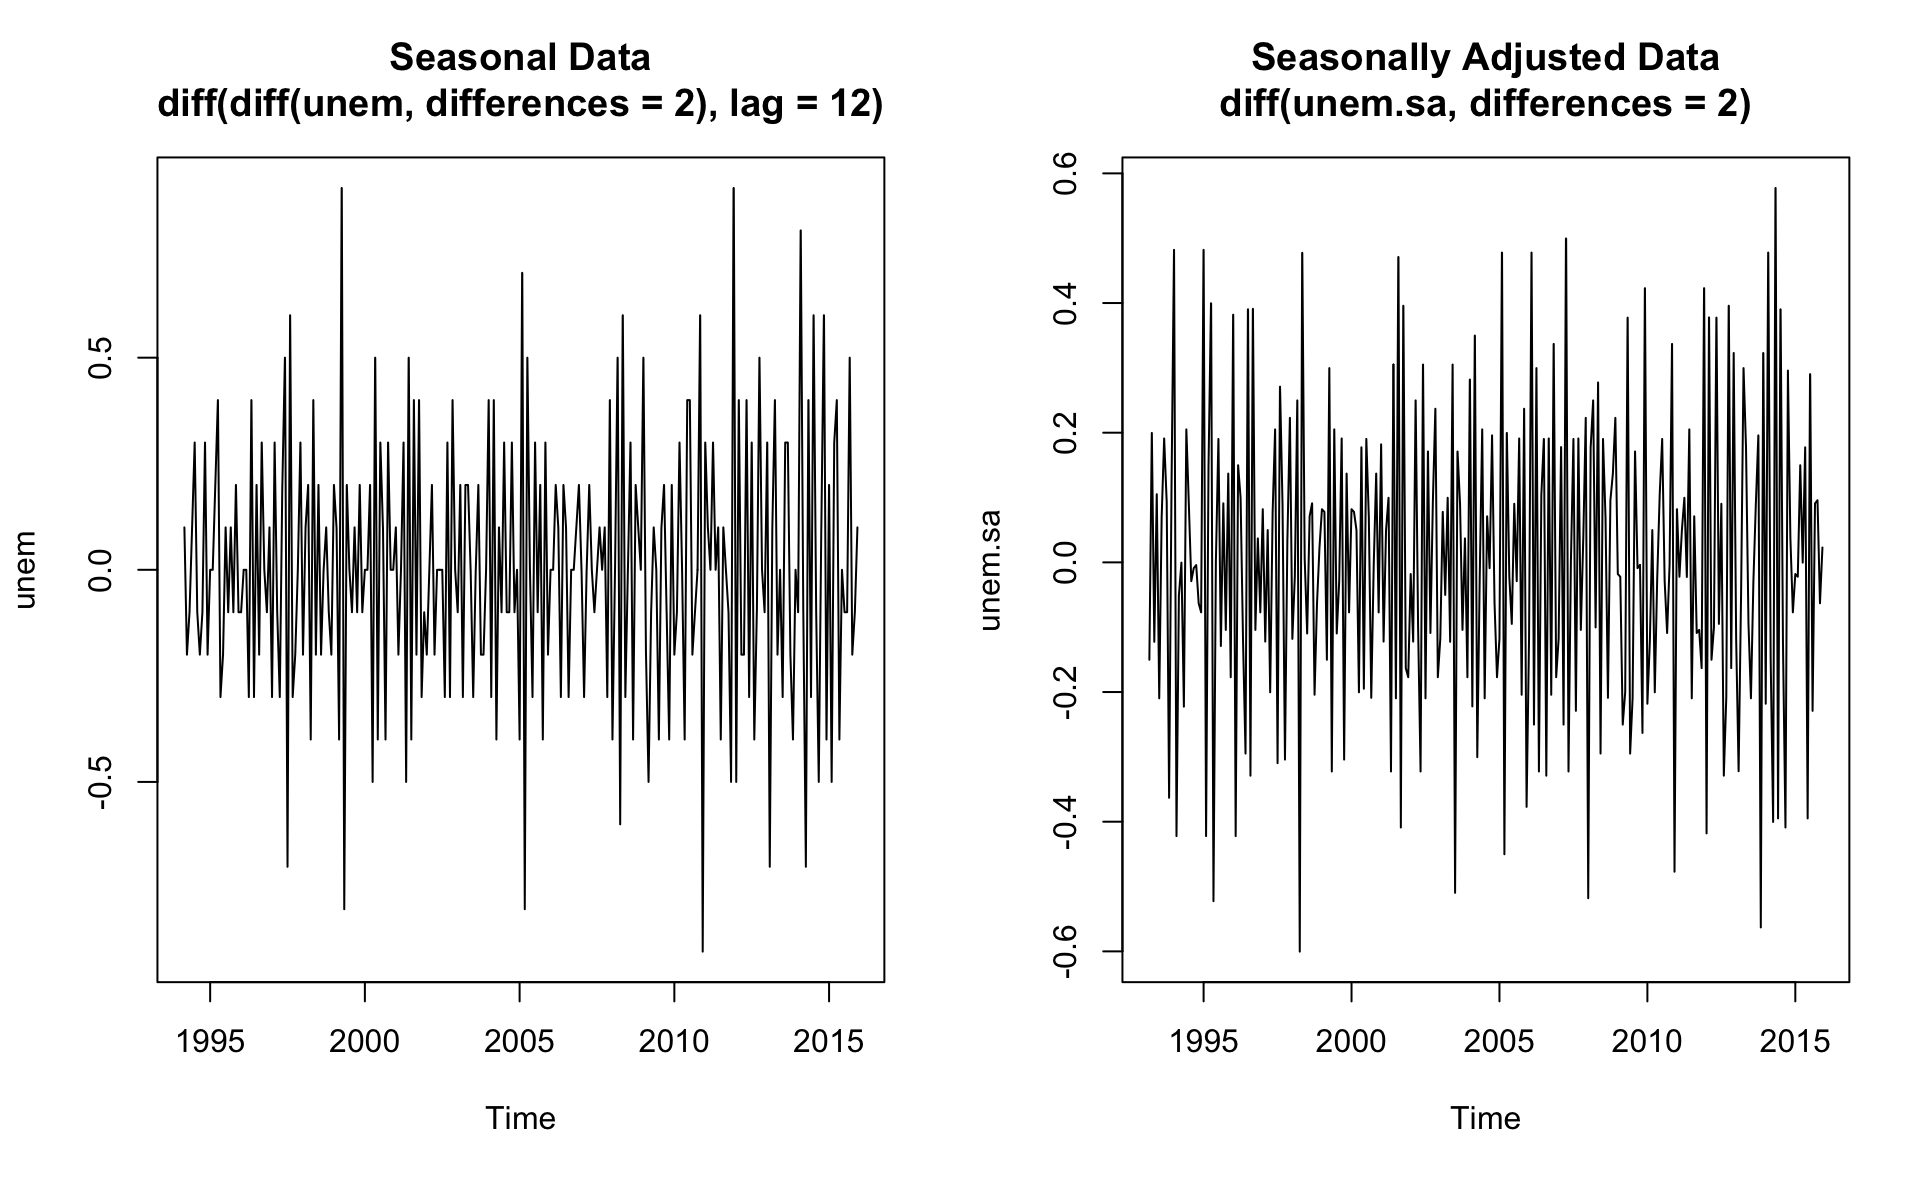
\includegraphics[width=\linewidth]{images/stationarity}
  \end{frame}
  
%-----------------------------------------------------------------------------------------
  
  \subsection{ACF \& PACF}
  \begin{frame}{ACF \& PACF Plots}
  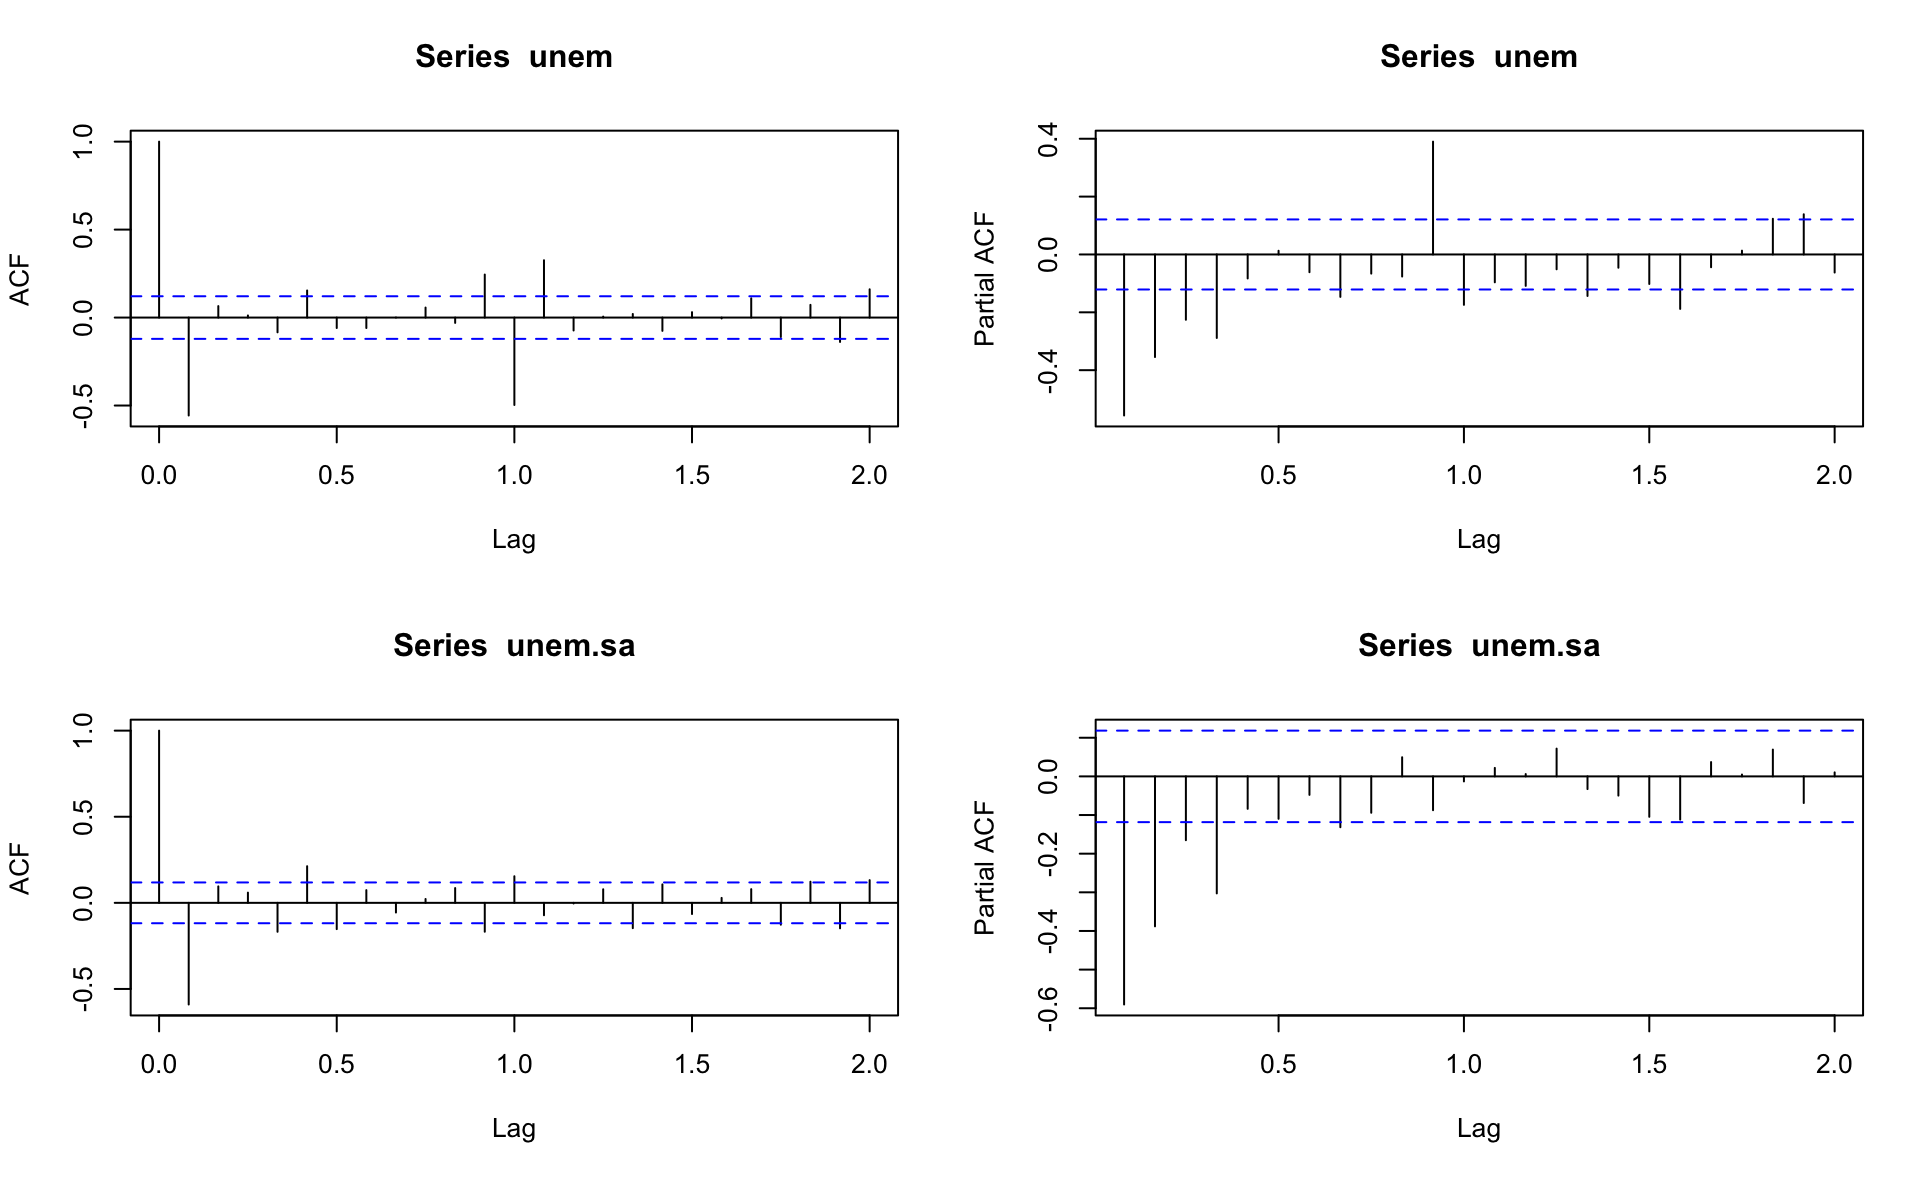
\includegraphics[width=\linewidth]{images/acfpacf}
  \end{frame}
 
%----------------------------------------------------------------------------------------- 

    \section{Model Comparisons}
    
%-----------------------------------------------------------------------------------------    
    \subsection{Overview}
  \begin{frame}{Models Considered}
    % latex table generated in R 3.2.4 by xtable 1.8-2 package
% Thu Jul  7 16:13:24 2016
\begin{table}[H]
\centering
\caption{Model Summaries}
\begin{tabular}{llccccc}
  \hline
 \textbf{\#}& \textbf{Data}  & \textbf{Order} & \textbf{Seasonal} & \textbf{XRegs} & \textbf{AIC} & \textbf{BIC} \\
 &&&\textbf{Order}&&&\\ 
  \hline
1 & Unem  & 0,2,1 & 1,1,0 & N & -2.27 & -3.23 \\ 
  2 & Unem  & 0,2,1 & 3,1,0 & N & -2.44 & -3.37 \\ 
  3 & Unem  & 4,2,1 & 3,1,0 & N & -2.44 & -3.32 \\ 
  4 & Unem.sa & 0,2,1 & 1,0,0 & N & -2.61 & -3.58 \\ 
  5 & Unem.sa  & 1,2,1 &  & N & -2.63 & -3.60 \\ 
  6 & Unem.sa & 0,2,1 & 1,0,0 & Y & -2.58 & -3.49 \\ 
  7 & Unem.sa  & 1,2,1 &  & Y & -2.60 & -3.49 \\ 
   \hline
\end{tabular}
\label{tab:models}
\end{table}
  \end{frame}
%-----------------------------------------------------------------------------------------

 \subsection{Seasonal Models}
 %-----------------------------------------------------------------------------------------
  \begin{frame}{Model 1: SARIMA\((0,2,1) \times (1,1,0)_{12}\)}
  		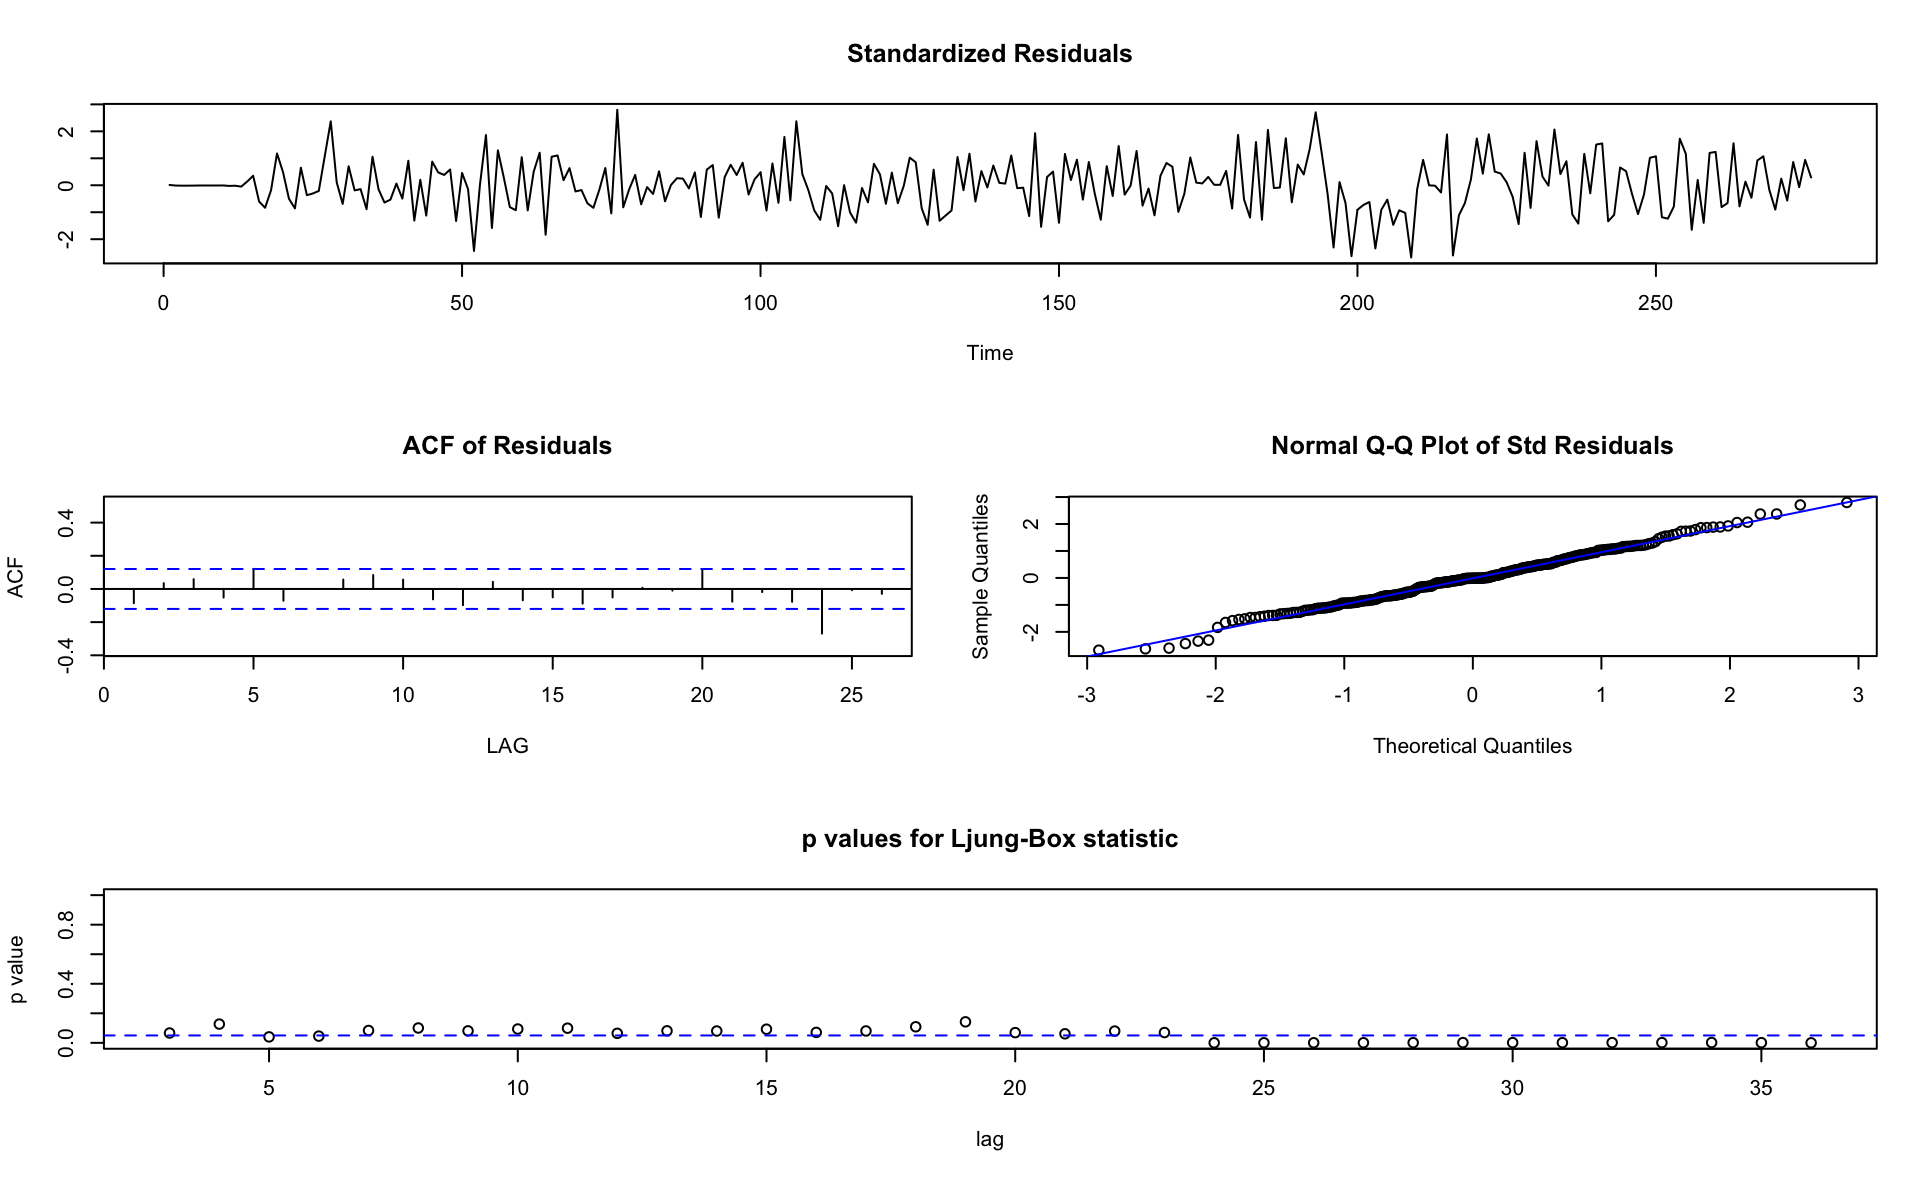
\includegraphics[width=\linewidth]{images/seasonalmodel1}
  \end{frame}

%-----------------------------------------------------------------------------------------

\begin{frame}{Model 2: SARIMA\((0,2,1) \times (3,1,0)_{12}\)}
  		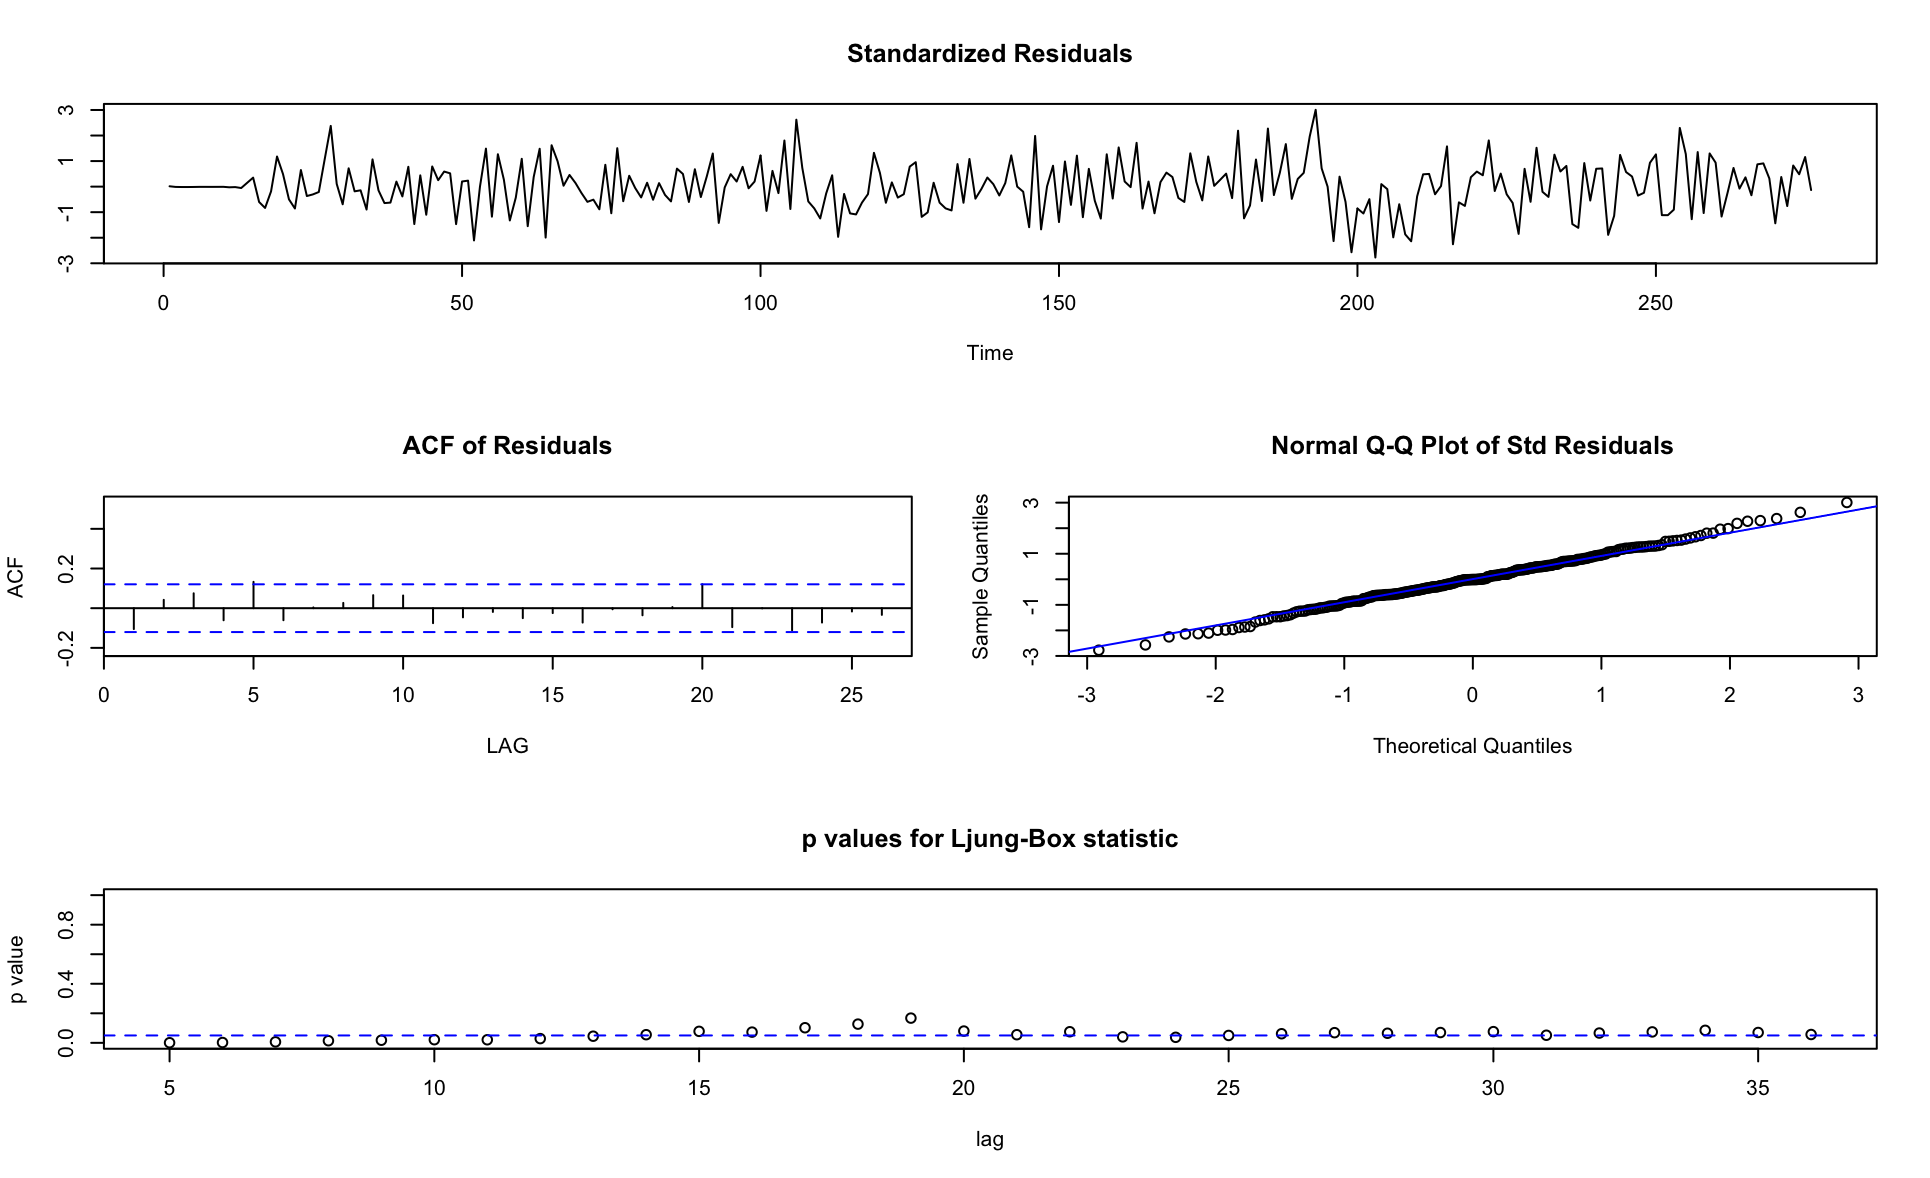
\includegraphics[width=\linewidth]{images/seasonalmodel2}
  \end{frame}  

%-----------------------------------------------------------------------------------------
  
  \begin{frame}{Model 3: SARIMA\((4, 2, 1) \times (3,1,0)_{12}\)}
  		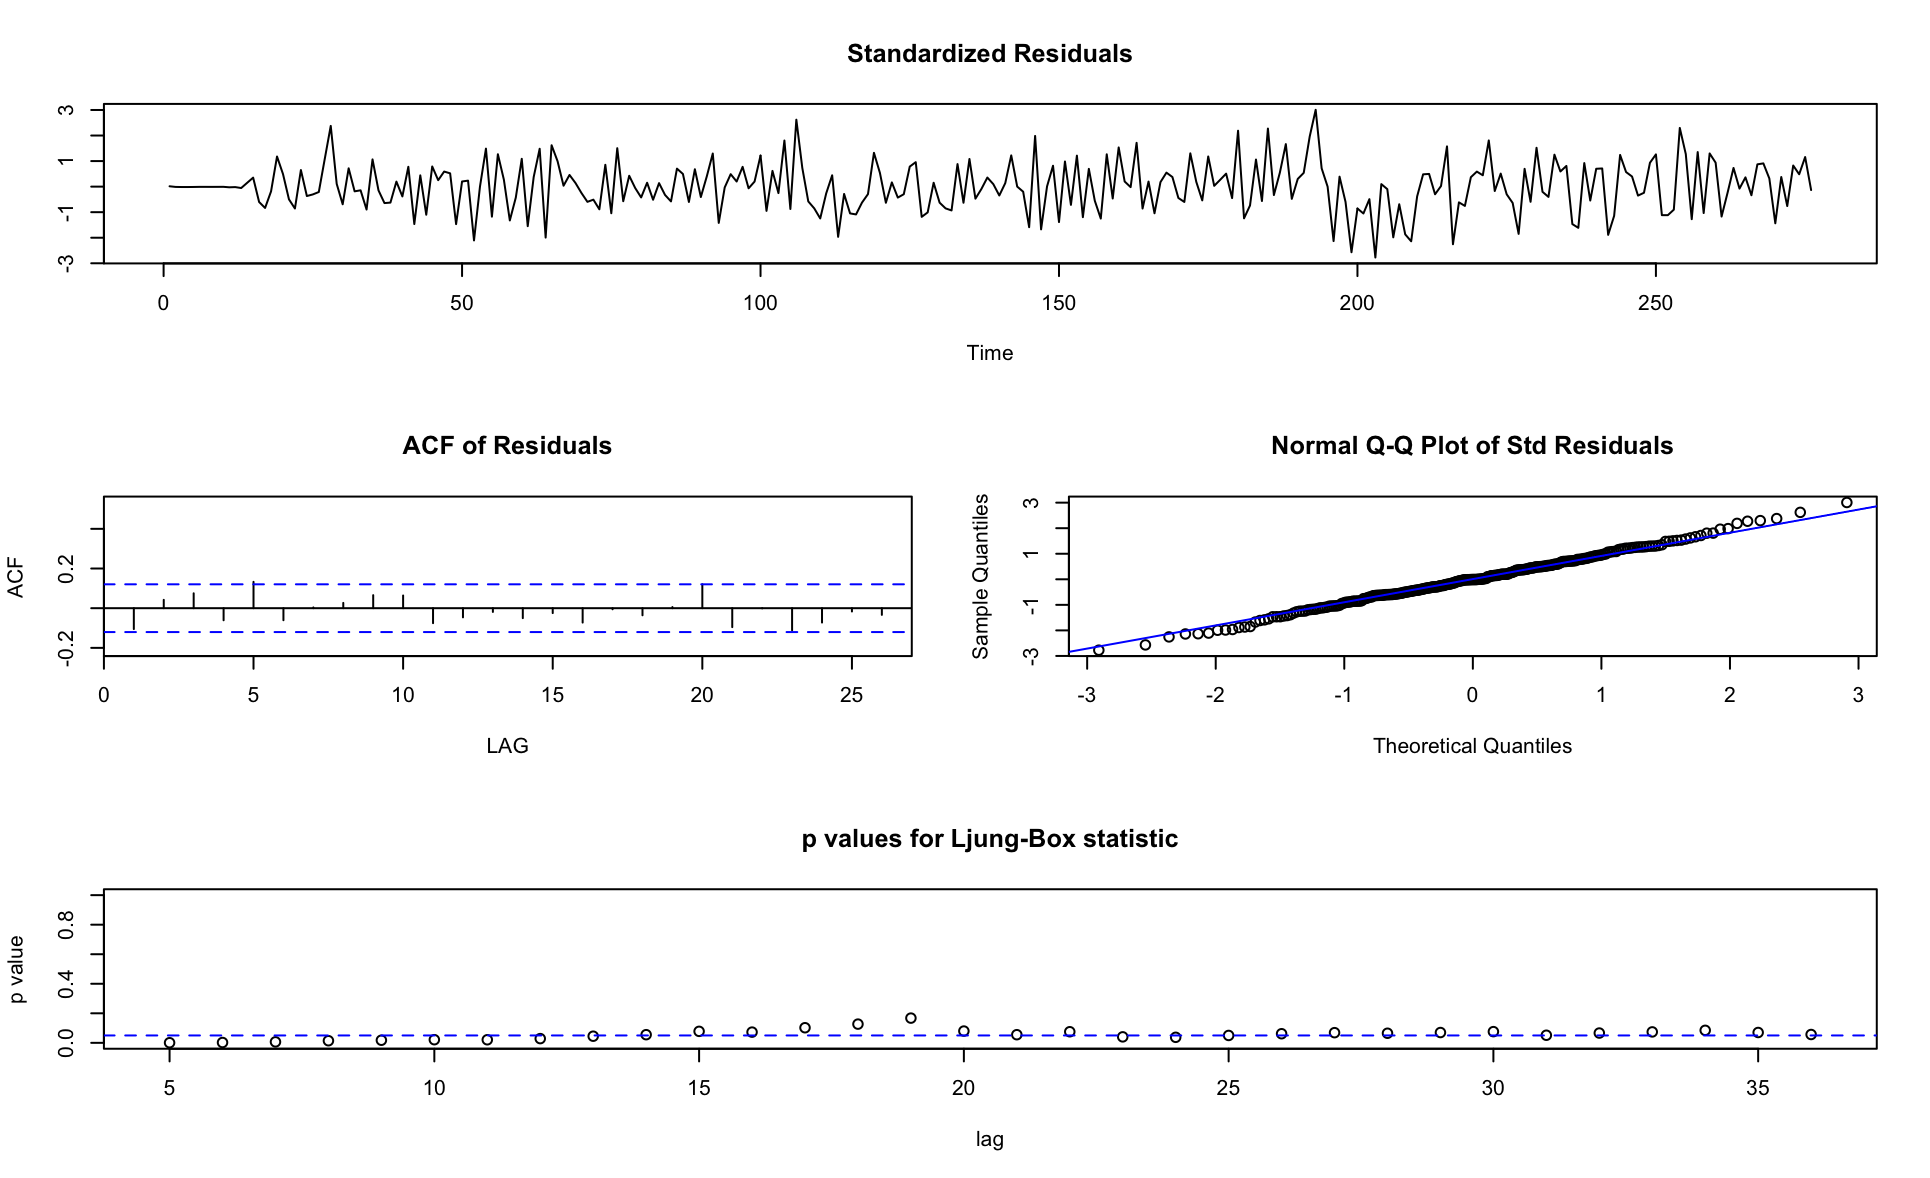
\includegraphics[width=\linewidth]{images/seasonalmodel3}
  \end{frame}  
%-----------------------------------------------------------------------------------------  

  \subsection{Seasonally Adjusted Models}
%-----------------------------------------------------------------------------------------  
  \begin{frame}{Model 4: SARIMA\((0,2,1) \times (1,0,0)_{12}\)}
  	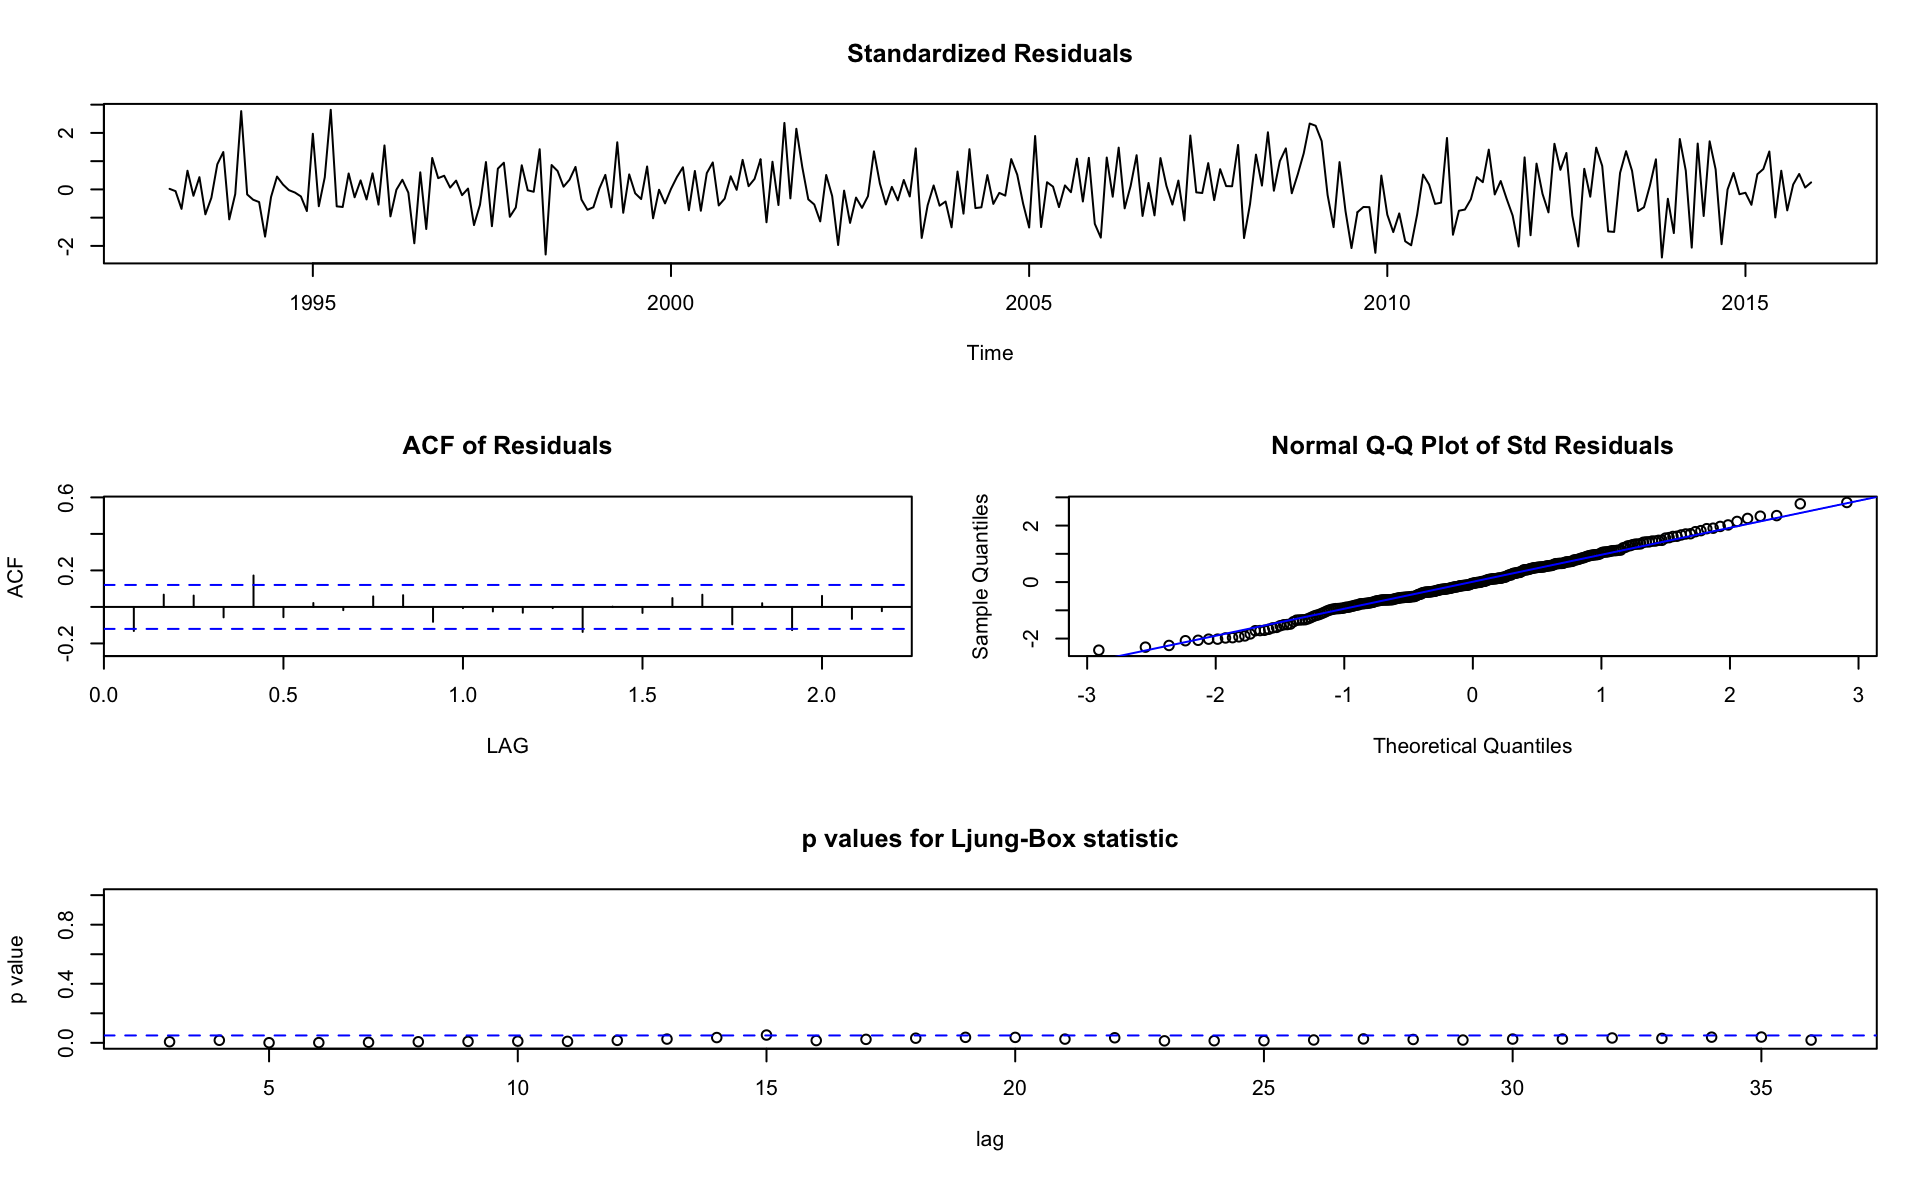
\includegraphics[width=\linewidth]{images/seasonallyadjustedmodel4}
  \end{frame}
  
%-----------------------------------------------------------------------------------------
  
  \begin{frame}{Model 5: ARIMA\((1,2,1)\)}
  		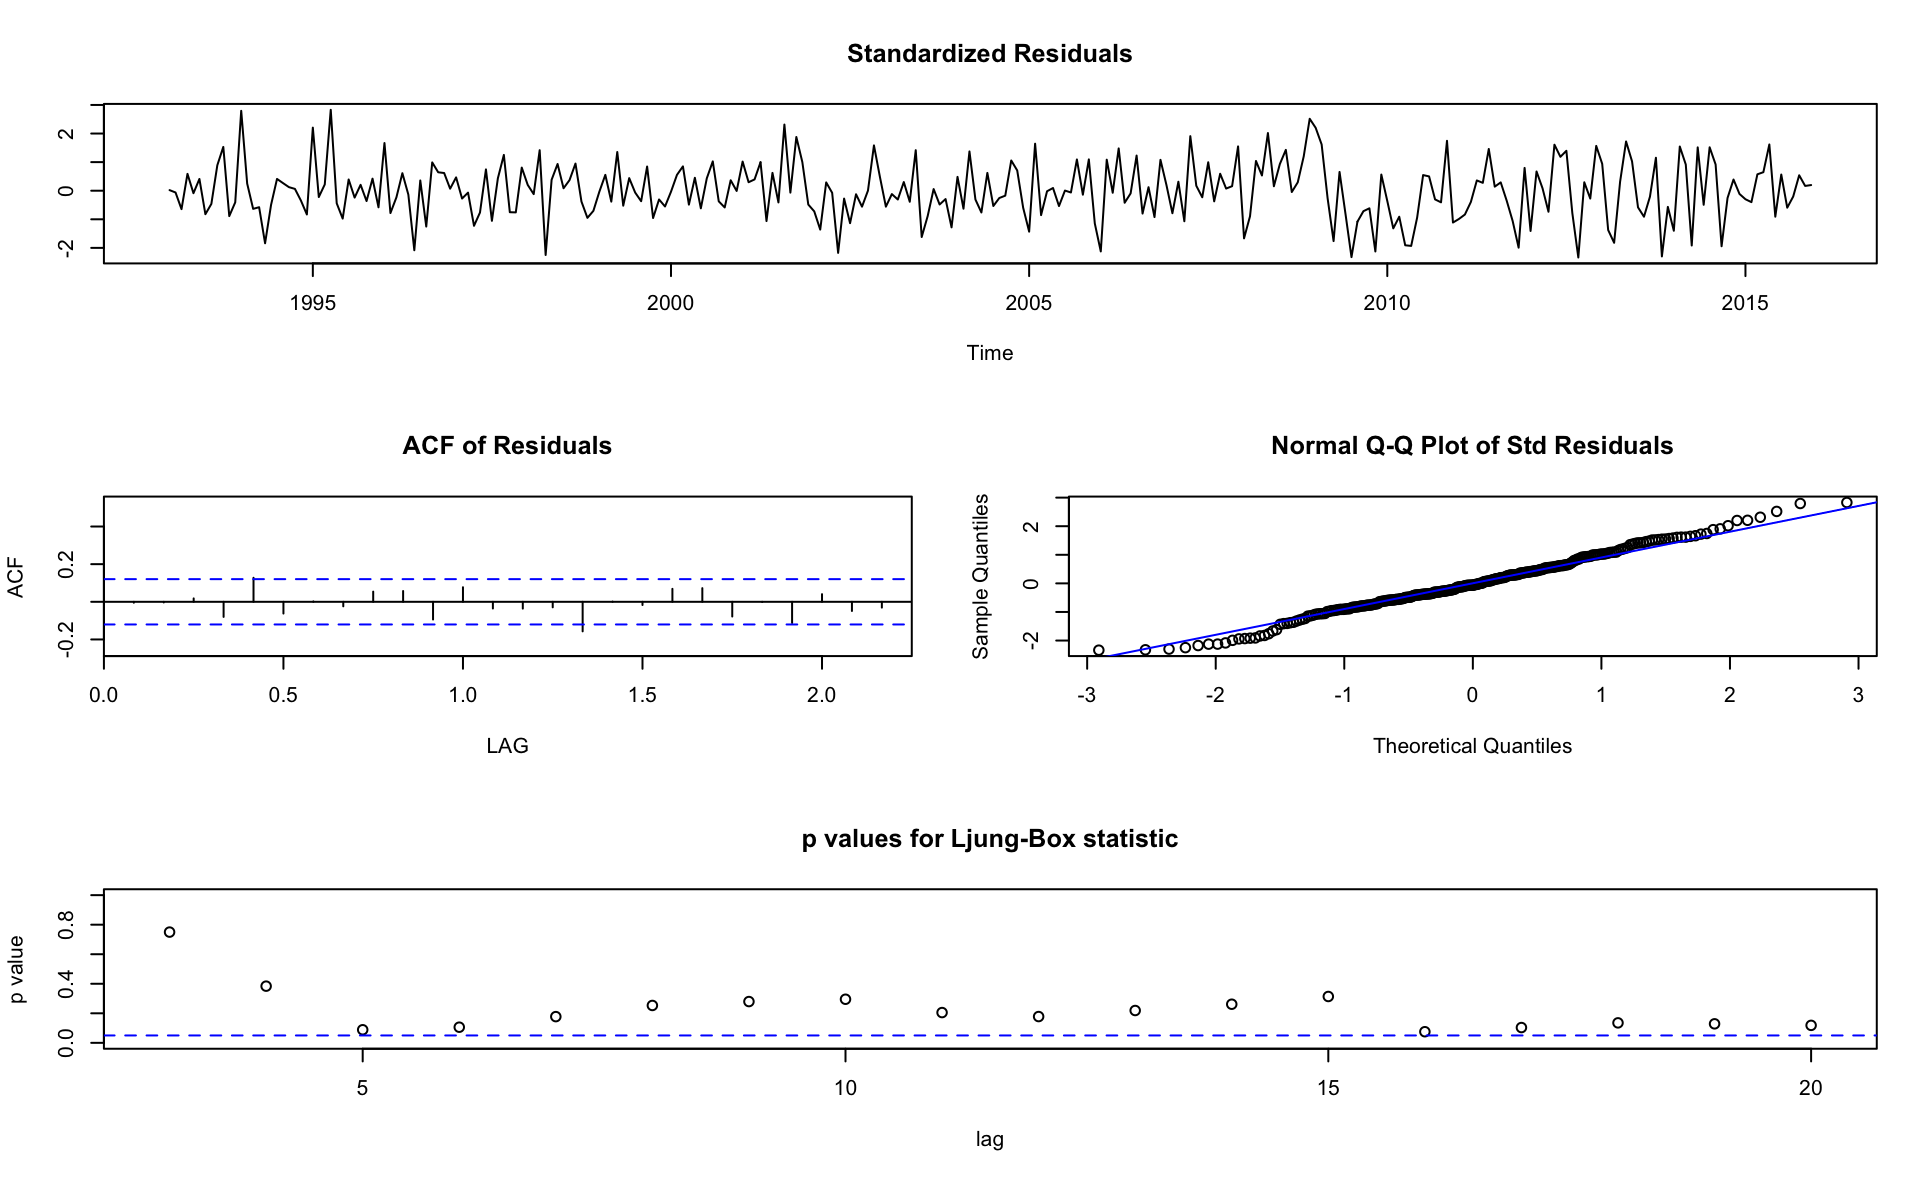
\includegraphics[width=\linewidth]{images/seasonallyadjustedmodel5}
  \end{frame}
  
  %-----------------------------------------------------------------------------------------
  
  \begin{frame}{Model 6: SARIMA\((0,2,1) \times (1,0,0)_{12}\) with Regressors}
  		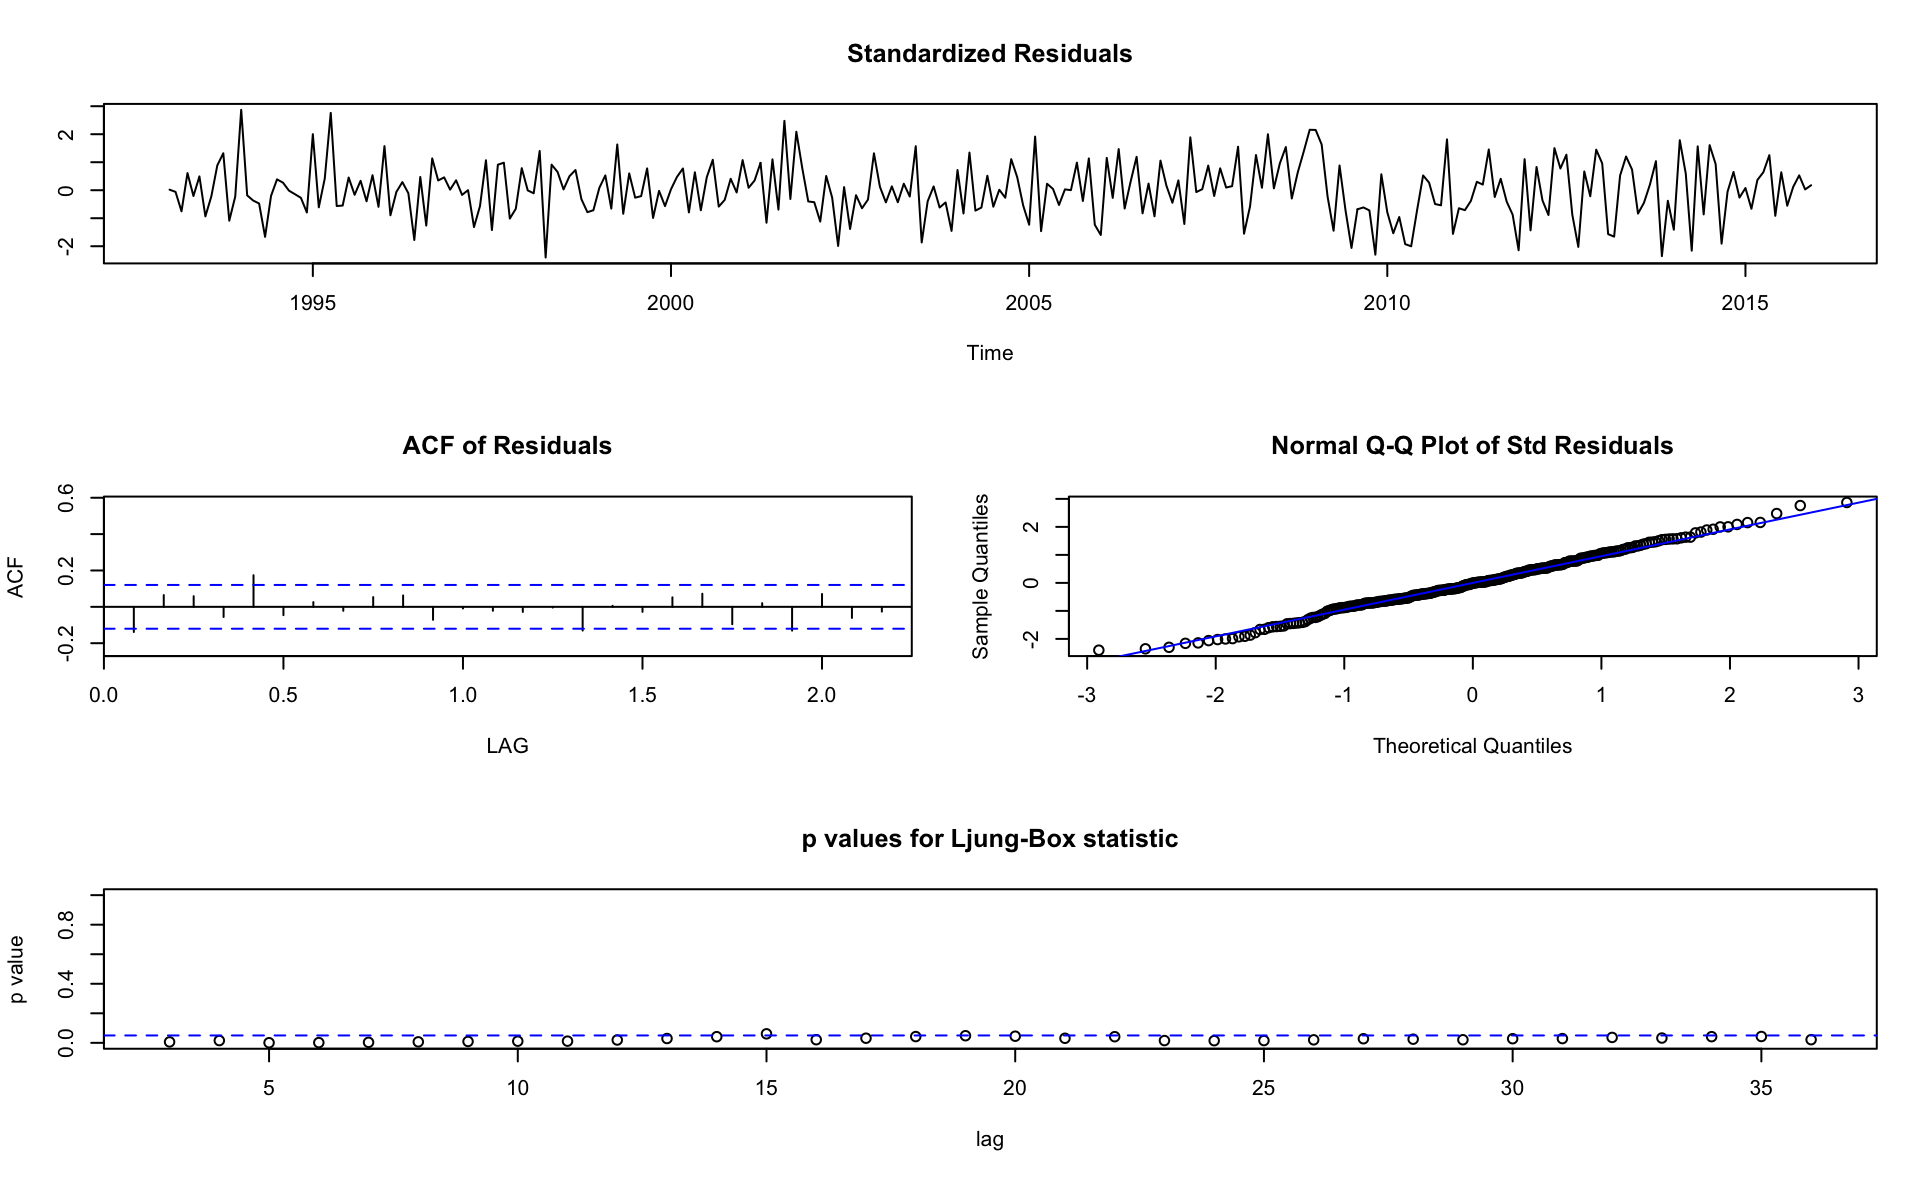
\includegraphics[width=\linewidth]{images/seasonallyadjustedmodel6}
  \end{frame}
  
  %-----------------------------------------------------------------------------------------
  
  \begin{frame}{Model 7: ARIMA\((1,2,1)\) with Regressors}
  		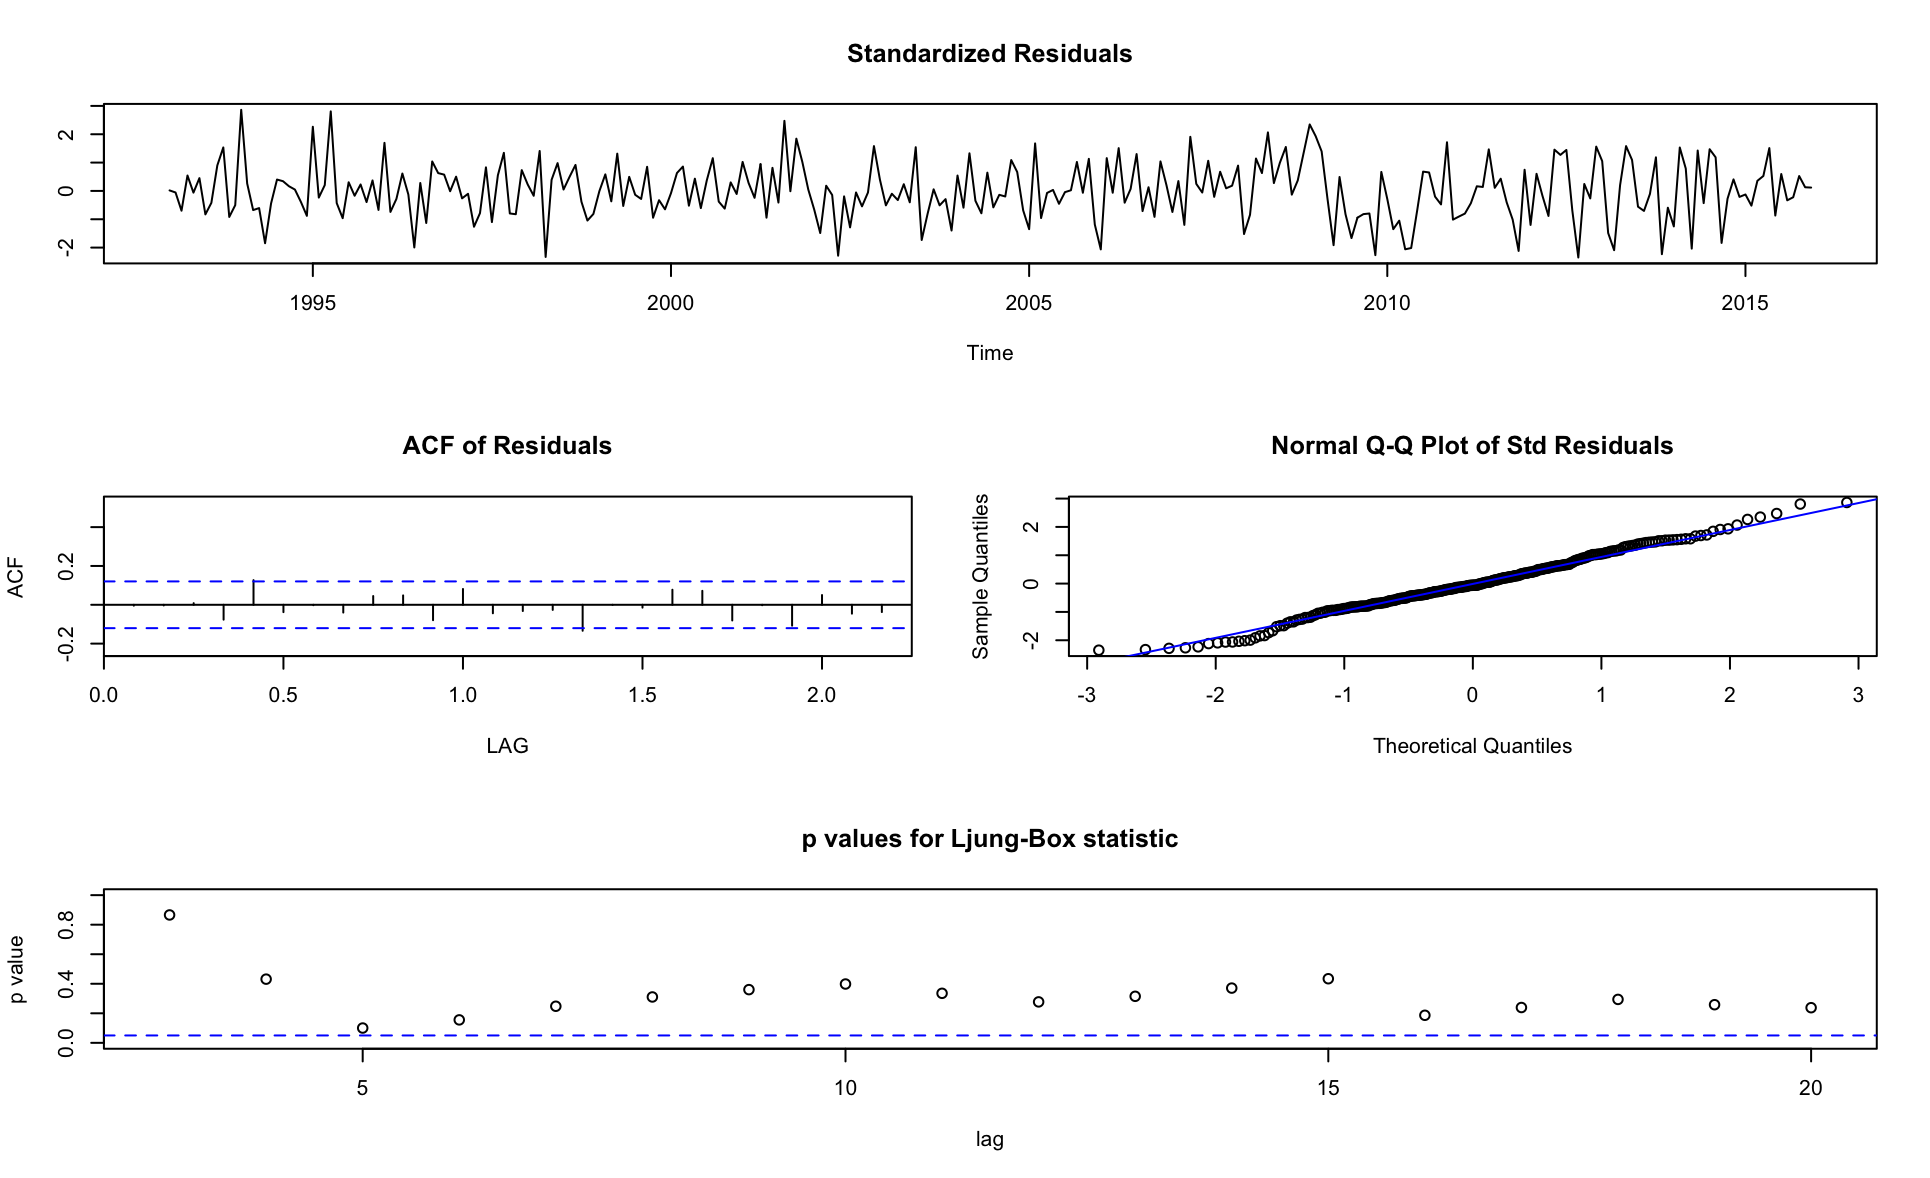
\includegraphics[width=\linewidth]{images/seasonallyadjustedmodel7}
  \end{frame}  
  
  %-----------------------------------------------------------------------------------------
  
\end{document}